\documentclass{beamer}
\usepackage{graphicx}

\usetheme{Frankfurt}
\setbeamertemplate{caption}[numbered]

\makeatletter
\newcommand\titlegraphicii[1]{\def\inserttitlegraphicii{#1}}
\titlegraphicii{}
\setbeamertemplate{title page}
{
  \vbox{}
   {\usebeamercolor[fg]{titlegraphic}\inserttitlegraphic\hfill\inserttitlegraphicii\par}
  \begin{centering}
    \begin{beamercolorbox}[sep=8pt,center]{title}
      \usebeamerfont{title}\inserttitle\par%
      \ifx\insertsubtitle\@empty%
      \else%
        \vskip0.25em%
        {\usebeamerfont{subtitle}\usebeamercolor[fg]{subtitle}\insertsubtitle\par}%
      \fi%     
    \end{beamercolorbox}%
    \vskip1em\par
    \begin{beamercolorbox}[sep=8pt,center]{author}
        \usebeamerfont{author}\insertauthor
    \end{beamercolorbox}
    \begin{beamercolorbox}[sep=8pt,center]{institute}
        \usebeamerfont{institute}\insertinstitute
    \end{beamercolorbox}
    \begin{beamercolorbox}[sep=8pt,center]{date}
      \usebeamerfont{date}\insertdate
    \end{beamercolorbox}%\vskip0.5em
  \end{centering}
  %\vfill
}
\makeatother

\title{Weather Prediction}
\subtitle{Will it rain Tomorrow?}
\author{Muhammed Berk Önder}
\institute{İstanbul Data Science Academy}
\date{\today}
\titlegraphic{
\includegraphics[width=15mm]{images/logo.png}}
\titlegraphicii{
\includegraphics[width=15mm]{images/logo.png}}

\begin{document}

\begin{frame}[plain]
    \maketitle

\end{frame}

\section{Introduction}
\begin{frame}[plain]
    \frametitle{Purpose}
    \LARGE{Will it rain tomorrow?}
    \normalsize
    \bigskip
    \begin{itemize}
        \item \textbf{Problem:} Can we tell from today that it will rain tomorrow? 
        \bigskip
        \item \textbf{Whom does it concern:} Anyone who doesn't want to get wet tomorrow.
    \end{itemize}
\end{frame}

\section{Methods}
\begin{frame}[plain]
    \frametitle{Methodology}
    \large
    \begin{itemize}
        \item Pull sql table from database with \textit{sqlalchemy}.
        \bigskip
        \item Analyse and Clean the data.
        \bigskip
        \item Used \textit{RandomForestClassifier} as a model.
        \bigskip
        \item Deploy with \textit{Flask}.
    \end{itemize}
\end{frame}

\section{Results}
\begin{frame}[plain]
    \begin{figure}
        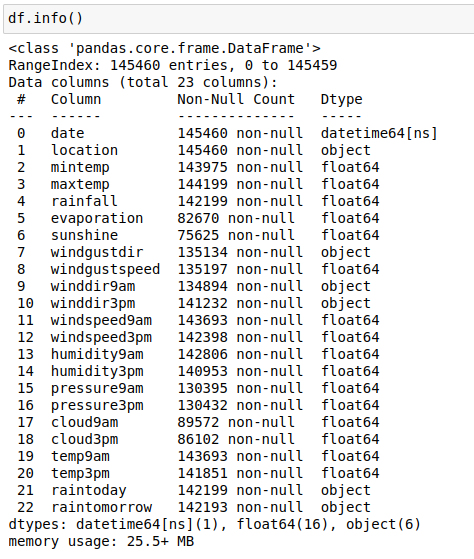
\includegraphics[width=.5\textwidth]{images/info.png}
    \end{figure}
\end{frame}

\section{Results}
\begin{frame}[plain]
    \begin{figure}
        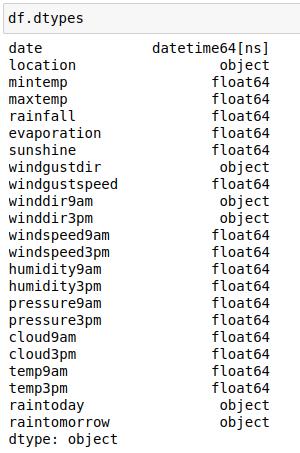
\includegraphics[width=.5\textwidth]{images/dtypes.png}
    \end{figure}
\end{frame}

\begin{frame}[plain]
    \begin{figure}
        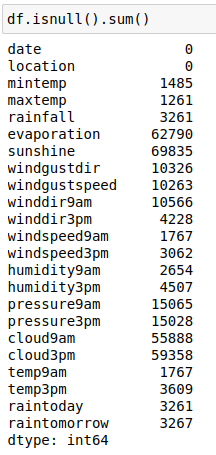
\includegraphics[width=.4\textwidth]{images/null.png}
    \end{figure}
\end{frame}

\begin{frame}[plain]
    \begin{figure}
        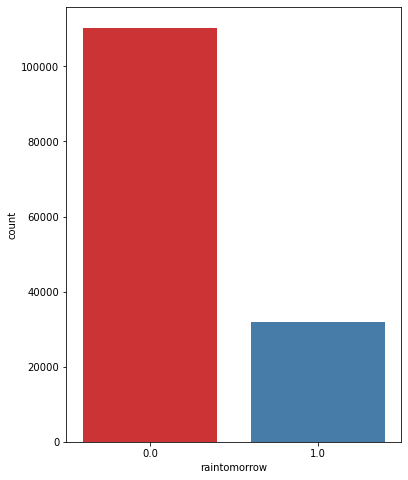
\includegraphics[width=.6\textwidth]{images/imbalance.png}
    \end{figure}
\end{frame}

\begin{frame}[plain]
    \begin{figure}
        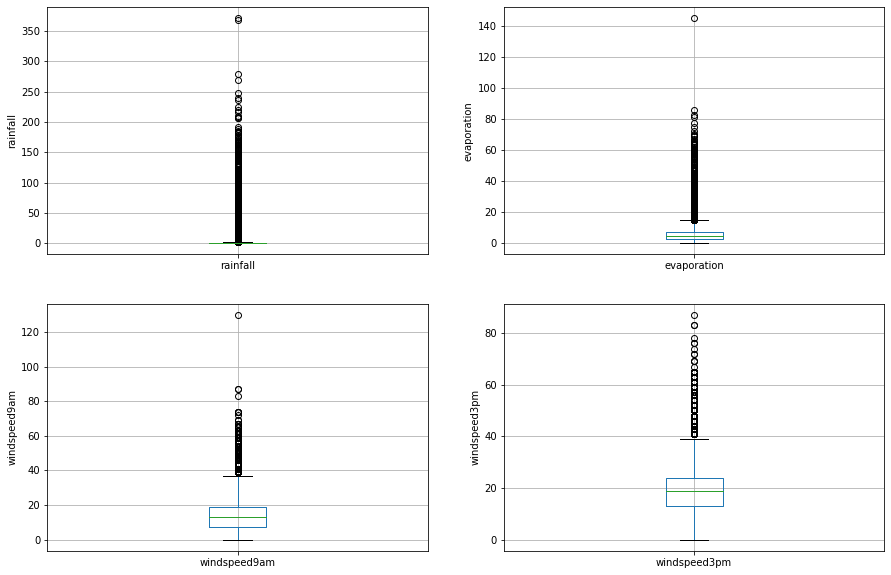
\includegraphics[width=\textwidth]{images/outliers.png}
    \end{figure}
\end{frame}

\begin{frame}[plain]
    \begin{figure}
        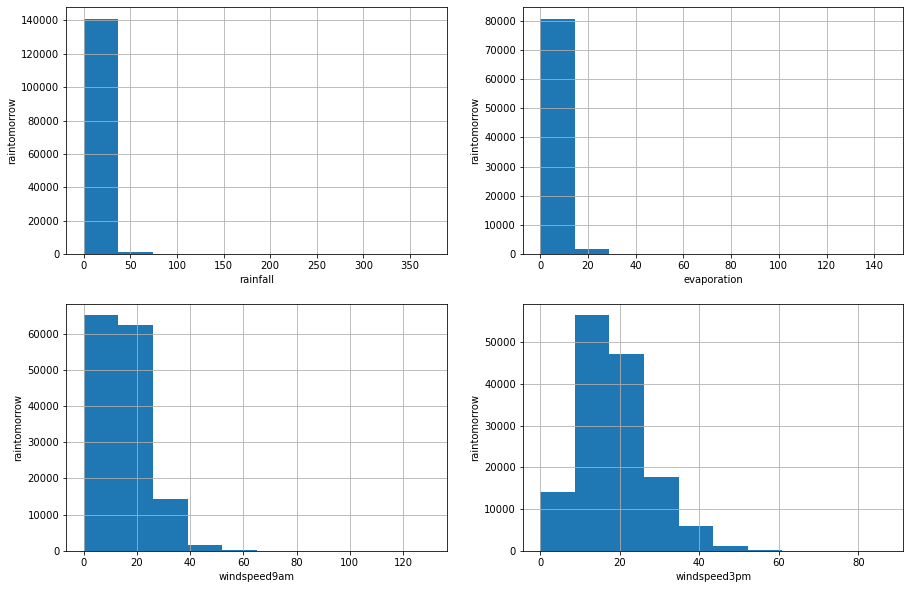
\includegraphics[width=\textwidth]{images/distribution.png}
    \end{figure}
\end{frame}

\begin{frame}[plain]
    \begin{figure}
        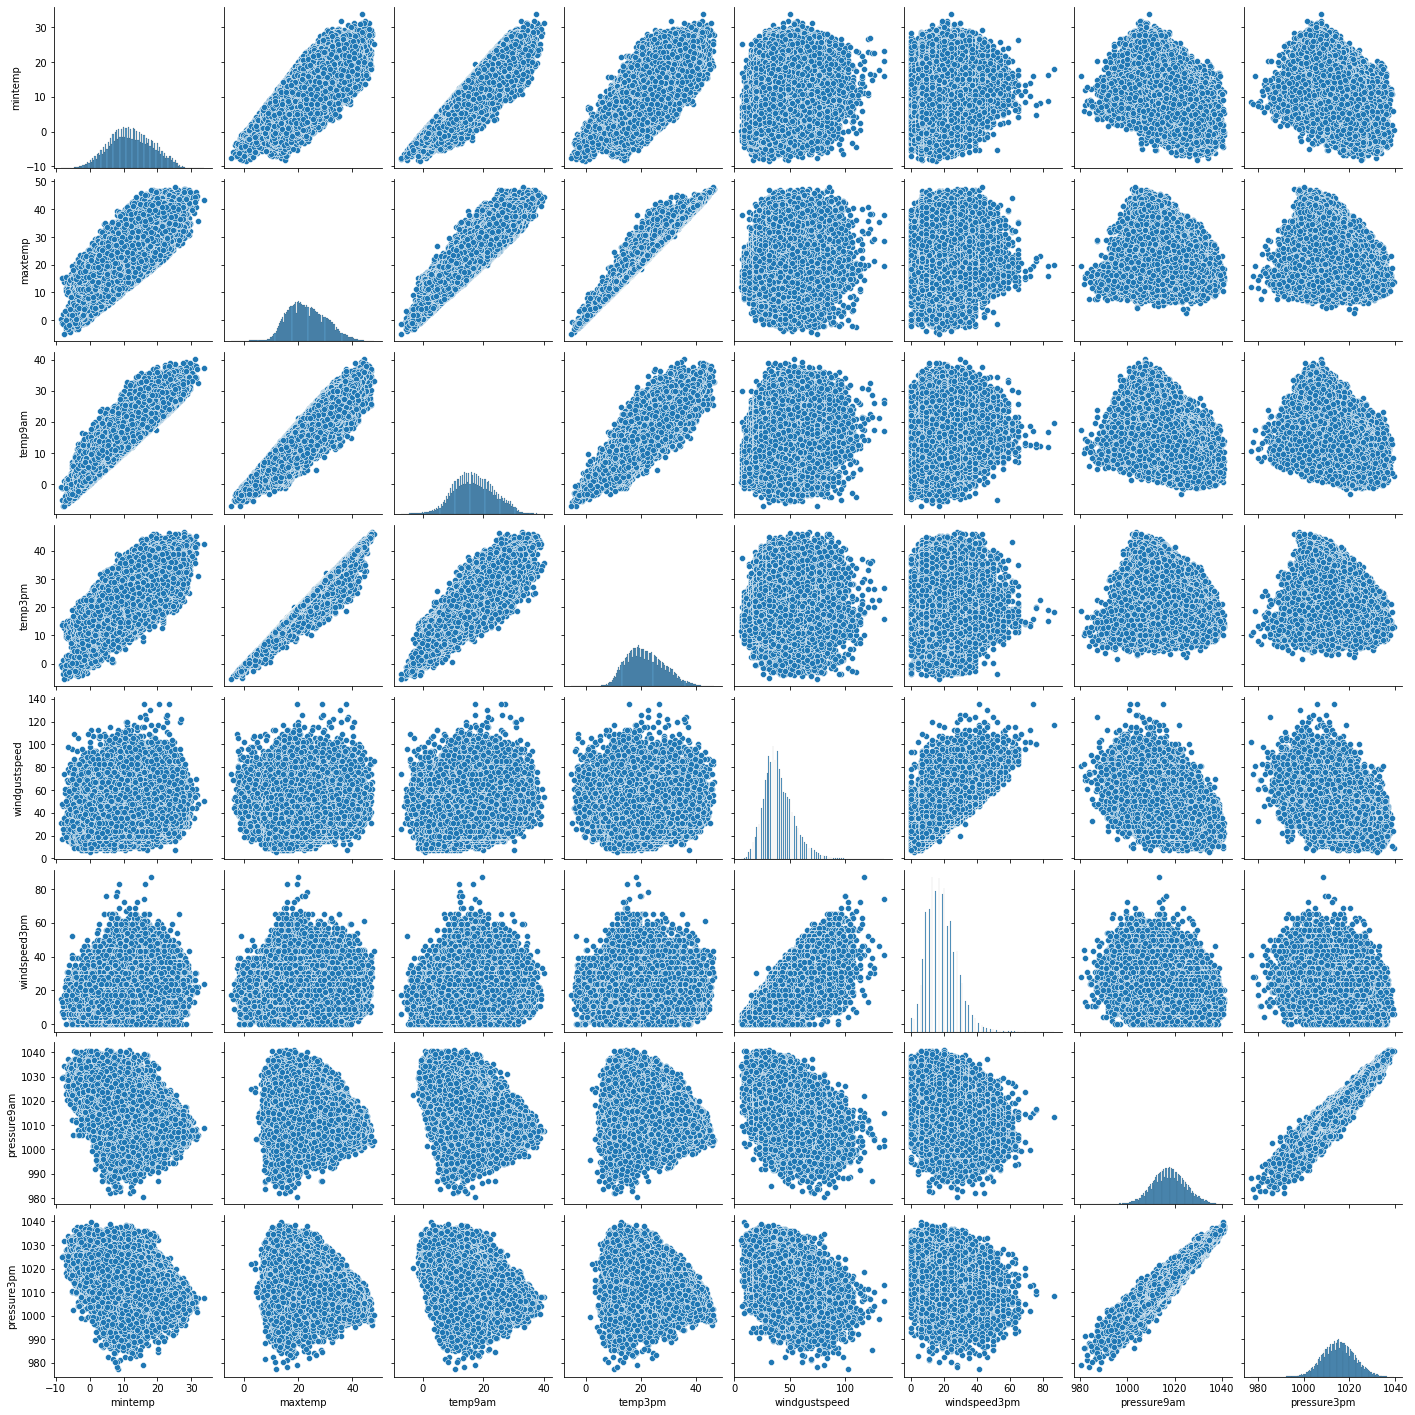
\includegraphics[width=.8\textwidth]{images/corr.png}
    \end{figure}
\end{frame}

\begin{frame}[plain]
    \begin{figure}
        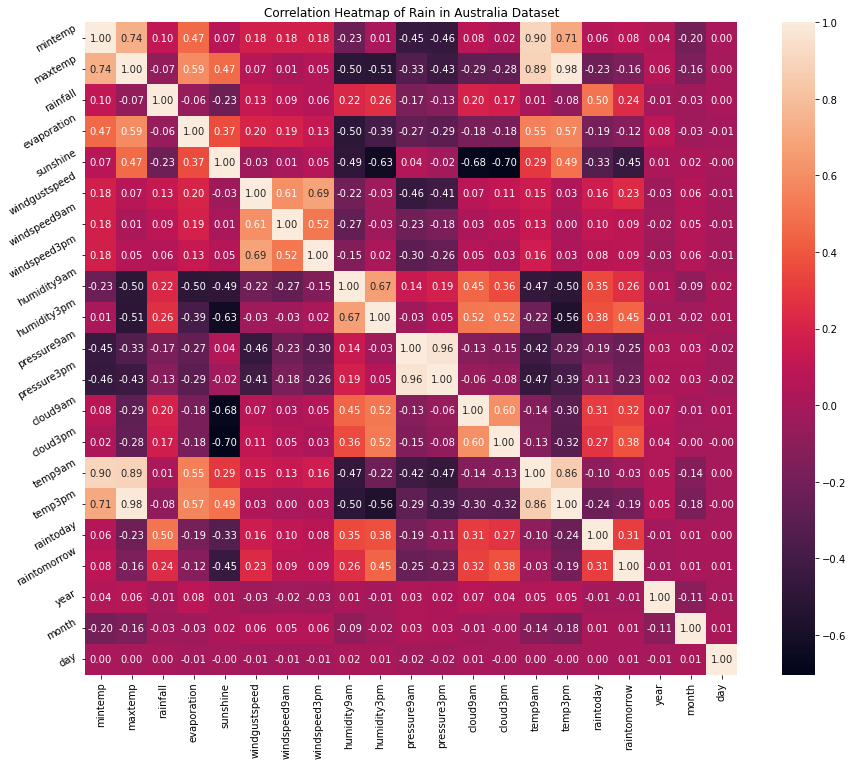
\includegraphics[width=.9\textwidth]{images/corr_heatmap.png}
    \end{figure}
\end{frame}

\begin{frame}[plain]
    From the above correlation heat map, we can conclude that:
    \small
    \begin{itemize}
        \item MinTemp and MaxTemp variables are highly positively correlated (correlation coefficient = 0.74).
        \item MinTemp and Temp3pm variables are also highly positively correlated (correlation coefficient = 0.71).
        \item MinTemp and Temp9am variables are strongly positively correlated (correlation coefficient = 0.90).
        \item MaxTemp and Temp9am variables are strongly positively correlated (correlation coefficient = 0.89).
        \item MaxTemp and Temp3pm variables are also strongly positively correlated (correlation coefficient = 0.98).
        \item WindGustSpeed and WindSpeed3pm variables are highly positively correlated (correlation coefficient = 0.69).
        \item Pressure9am and Pressure3pm variables are strongly positively correlated (correlation coefficient = 0.96).
        \item Temp9am and Temp3pm variables are strongly positively correlated (correlation coefficient = 0.86).
    \end{itemize}
\end{frame}

\begin{frame}[plain]
    \begin{figure}
        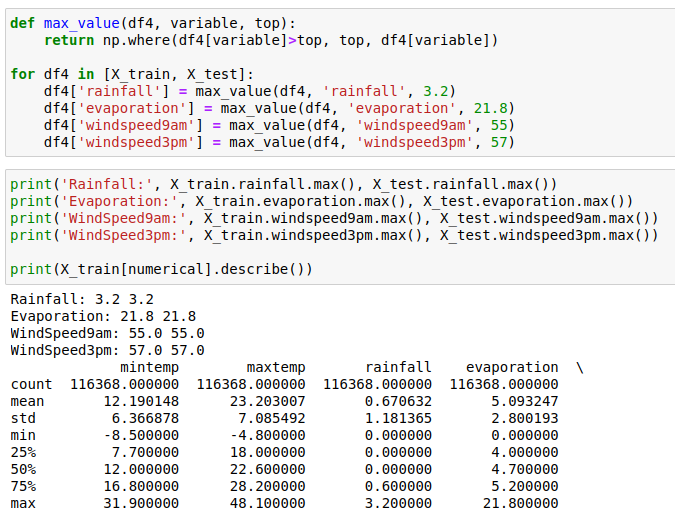
\includegraphics[width=\textwidth]{images/max_value.png}
    \end{figure}
\end{frame}

\begin{frame}[plain]
    \begin{figure}
        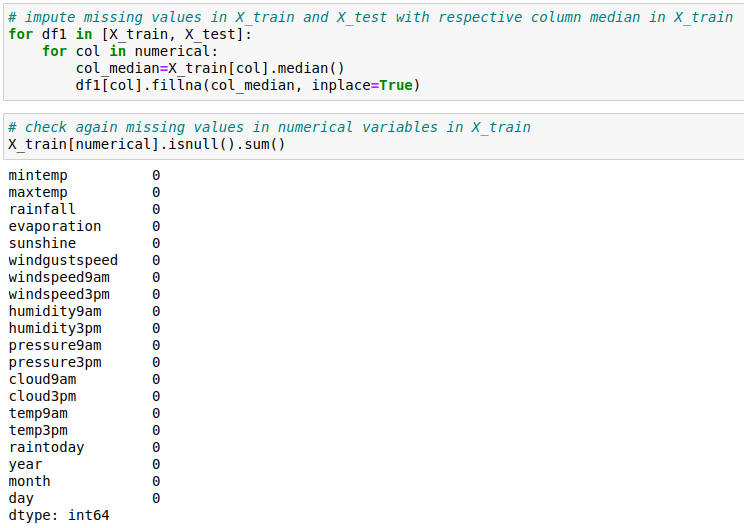
\includegraphics[width=\textwidth]{images/impute_numerical.png}
    \end{figure}
\end{frame}

\begin{frame}[plain]
    \begin{figure}
        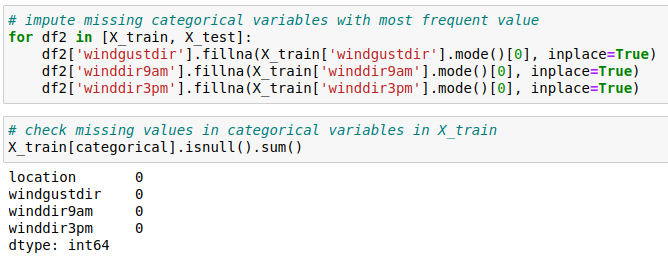
\includegraphics[width=\textwidth]{images/impute_mode.png}
    \end{figure}
\end{frame}

\begin{frame}[plain]
    \begin{figure}
        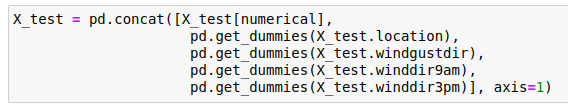
\includegraphics[width=\textwidth]{images/get_dummies.png}
    \end{figure}
\end{frame}

\begin{frame}[plain]
    \begin{figure}
        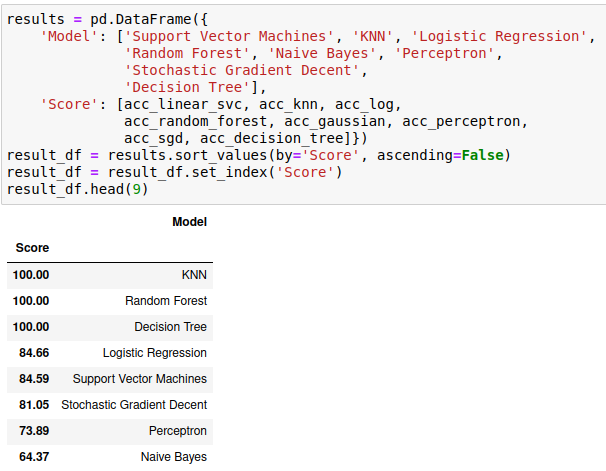
\includegraphics[width=\textwidth]{images/best_model.png}
    \end{figure}
\end{frame}

\begin{frame}[plain]
    \begin{figure}
        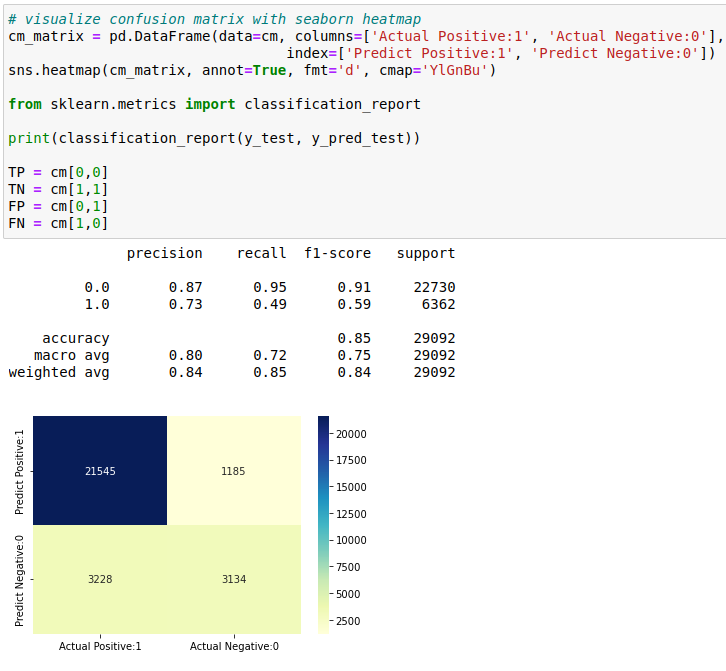
\includegraphics[width=.9\textwidth]{images/confusion_heatmap.png}
    \end{figure}
\end{frame}

\end{document}